\section{Progettazione}
	
  \subsection{Design}
  Per il design del sito, sono state perseguite due principali strade:
  \begin{itemize}
    \item \textit{Desktop First}: il nostro sito si rivolge ad un utenza molto tecnica e pensiamo che l'utilizzo del sito avverrà principalmente da Desktop. Viene comunque data importanza all'utenza che deciderà di approcciarsi a questo sito tramite smartphone.
    \item \textit{Layout a 4 Pannelli}: utilizzato in tutte le pagine del sito tranne UserProfile, dove viene utilizzato un Layout a 5 Pannelli, aggiungendo una \textbf{Sidebar} per la navigazione tra le sottopagine di User Profile.
  \end{itemize}

  I 4 pannelli che compongono il layout delle nostre pagine sono:
  \begin{enumerate}
    \item \textbf{Header}: composto dal logo del sito e dai link alle altre pagine;
    \item \textbf{Breadcrumb}: contiene i Link alle pagine "precedenti" a quella che si sta attualmente visitando; il breadcrumb è di vitale importanza per far sì che l'utente
      non si senta perso nella navigazione del sito. Nel caso del nostro sito, il breadcrump è stato scritto in maniera da simulare un path di un filesystem;
    \item \textbf{Main}: corrisponde al vero e proprio contenuto della pagina;
    \item \textbf{Footer}: contiene informazione su come contattare l'Admin in caso di problemi e il link per le FAQ.
  \end{enumerate}
  
  Il quinto pannello, ovvero la \textbf{sidebar}, è utilizzato nella pagina UserProfile. 
  Questa pagina raccoglie informazioni utili dell'utente $($informazione su utente, sui lavori svolti e proposti$)$, la possibilità di modificare i propri dati utente ed è accessibile solo dallo stesso utente.


  \subsection{Database}
  Il database risulta essere una parte cruciale del nostro sito, poiché il contenuto principale di molte pagine viene creato in base ai risultati presenti su quest'ultimo. 
  \begin{figure}[h]
    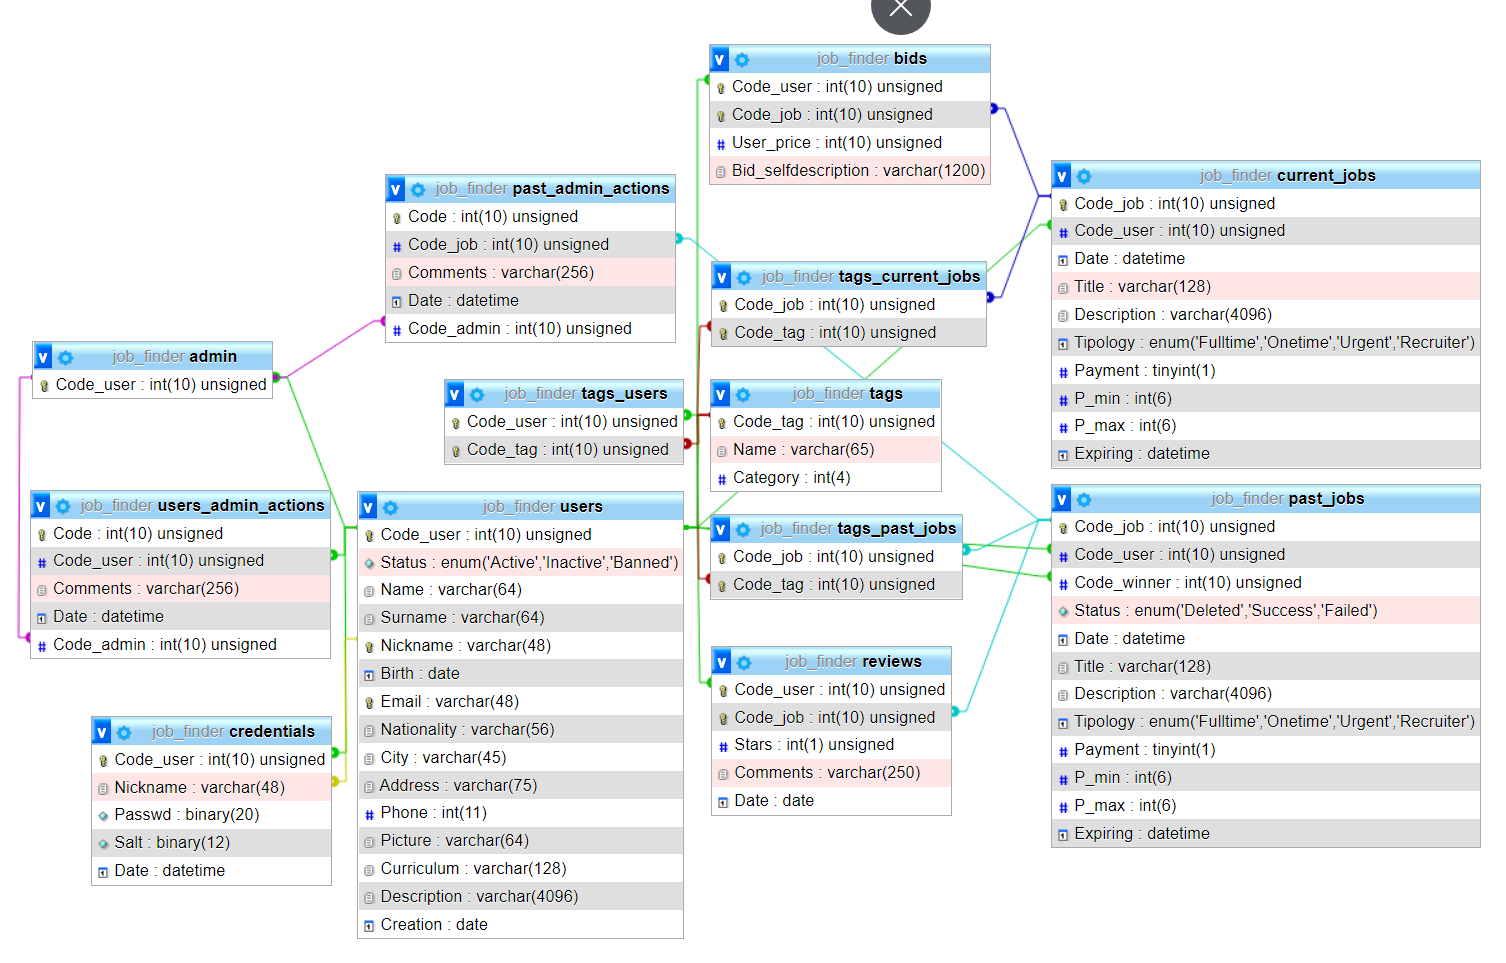
\includegraphics[scale=0.5]{Images/DB2.png}
    \caption{Schema del database}
    \centering
  \end{figure}
  Le tabelle che compongono il nostro sono :
  \begin{itemize}
    \item \textbf{users e credentials} : users contiene i dati utente e Credentials contiene le credenziali, questi dati sono divisi in due tabelle per evitare leak di informazioni;
    \item \textbf{current\textunderscore jobs e bids} : current\textunderscore job contiene i dati inerenti alle offerte di lavoro, bids contiene i dati inerenti alle candidature per le offerte in questione;
    \item \textbf{past\textunderscore jobs e reviews} : past\textunderscore jobs contiene i dati inerenti alle offerte di lavoro eliminate, fallite o avvenute con successo; reviews contiene i feedback delle past\textunderscore jobs avvenute con successo;
    \item \textbf{tags, tags\textunderscore users, tags\textunderscore past\textunderscore jobs, tags\textunderscore current\textunderscore jobs} : tags contiene tutti i possibili tag presenti nel sito, tags\textunderscore users, tags\textunderscore past\textunderscore jobs e tags\textunderscore current\textunderscore jobs contengono le chiavi delle rispettive tabelle e di tags per associare le due tabelle;
    \item \textbf{admin, user\textunderscore admin\textunderscore actions e past\textunderscore admin\textunderscore actions} : admin contiene i code\textunderscore user degli utenti admin, le tabelle user\textunderscore admin\textunderscore actions e past\textunderscore admin\textunderscore actions contengono rispettivamente gli storici delle azioni eseguite dagli admin su utenti e su offerte di lavoro. 
  
  \end{itemize}

  Viene utilizzato PHP per interrogare il database, tramite una classe specializzata chiamata DBAccess.php. \\
  Molte pagine all'interno del nostro sito vengono riempite dinamicamente con i risultati forniti dal database, 
  alcuni esempi possono essere la ricerca dei lavori su findJob, la quale utilizza sia PHP che AJAX, o le visualizzazione dei dati degli utenti di ViewUser.

  

  \subsection{Obiettivi}
  Il gruppo si è prefissato alcuni obiettivi da perseguire durante la realizzazione di questo progetto, al fine di mantenere l'accessibilità e l'usabilità come priorità e migliorare il più possibile l'esperienza utente :
  \begin{itemize}
    \item utilizzo di tag \textit{alt} per tutte le immagini presenti nel sito. Questo non è utile solamente quando l'immagine non è disponibile, ma inoltre risulta essere fondamentale poiché è cio che viene letto dagli screen reader, quindi elemento necessario se si vuole fornire la possibilità ad un utente che utilizza questo strumento di comprendere il contesto o il significato di un'immagine.
        Esistono alcuni casi in cui \textit{alt} viene inserito con valore vuoto, questo per due motivi :
    \begin{itemize}
      \item l'immagine è associata ad un link, come nel caso dei link dell'header. In questo caso, aggiungere un tag che ripeta il significato del link viene considerata bad practise poiché l'utente che utilizza screen reader dovrà ascoltare due volte lo stesso elemento e l'utente che si ritrova con l'immagine non disponibile si troverà con una scritta "raddoppiata", creando confusione;
      \item l'immagine è di contesto, non ha un significato specifico o importanza a livello di contenuto; viene quindi tenuto alt vuoto.
    \end{itemize}
    \item reinserimento automatico degli input inseriti dall'utente quando avviene il reindirizzamento della pagina sulla stessa 
     $($es: il submit della form di createJob richiama createJob.php che, controllato i dati e confermando un possibile errore, rimanda alla pagina createJob ma ricaricando i valori correttamente inseriti $)$;
    \item uso intelligente del \textit{breadcrumb}, poiché il breadcrumb fornisce informazione all'utente su come é arrivato su quella parte del sito, è fondamentale che il breadrcumb risulti completo;
    \item meccanismi di \textit{hidden help} e \textit{gobacktothetop}, entrambi meccanismi che utilizzano $<$a href="\#"$>$ per condurre l'utente su diversi elementi della pagina. I primi vengono utilizzati da utenti che utilizzano screen reader, i secondi vengono utilizzati quando le pagine risultano verticalmente troppo estese eq quindi faticose nel tornare all'inizio della pagina;
    \item aiuti utente e indicazione sulle correzioni di errori nell'inserimento dati. Nel caso in cui avvengano degli errori, quali mancanza di input o altre tipologie di errori, verranno riportati i cambiamenti da attuare ed il motivo dell'errore, in modo da aiutare l'utente a inserire i dati correttamente.
  \end{itemize} 